% Worksheet
% NOTE: For two marks complete and hand-in Pages 7-8 before the end of the lab.
% You are a design engineer working at a large automotive component manufacturer. You 
% have been asked to design a system to monitor the air intake filter on an engine. You are 
% to devise a system that will determine if the air filter is properly installed or damaged and
% when the filter is clogged, which will turn on the engine warning light, so that the driver 
% knows that the filter will need to be replaced. 
% When a clean filter is installed, the pressure drop across the filter is 0.7 kPa when the 
% engine is at idle. (The pressure drop is the differential pressure between the air upstream 
% and downstream of the filter). If a filter has a leak due to damage or improper installation, 
% then the pressure drop will be lower than 0.7 kPa. For example, the pressure drop will be 
% zero if no filter is installed. Also, as debris is collected on the filter the pressure drop 
% increases. The filter should be replaced when the pressure drop reaches 0.9 kPa when the 
% engine is at idle. Thus, it is desired to measure pressure drops from 0 to 0.9 kPa.
% The analog signal from the pressure transducer will be read by the vehicle’s engine 
% control unit (ECU). The ECU uses a 12-bit A/D converter and accepts 0–5 V input 
% voltage.
% Your supervisor told you to use a sensor from Honeywell (see data sheet posted on 
% eClass) that measures differential pressure with the model number: 
% ABP2 D DA D XXXXX A A Y, where XXXXX is a place holder for the pressure range, 
% and Y is a place holder for the supply voltage (either 3.3 V or 5 V). See Page 10 of the 
% data sheet to understand the model number. 
% Recommend a system to monitor the pressure drop by completing the following steps:
% 1) See Page 10 of the data sheet and select a pressure range in kPa which is 
% suitable for your application. [1 mark]. Why did you choose that range? [1 
% mark].
% 2) See Page 6 of the data sheet. The output of the sensor depends on the supply 
% voltage of the sensor. Plot the expected voltage output of your sensor as a 
% function of pressure over the range of the sensor if the supply voltage is 3.3 V 
% and if it is 5V. Put both lines on the same plot. [2 marks]. Calculate the 
% sensitivity of the sensor for each supply voltage. [1 mark]
% 3) The ECU uses 12-bit A/D converters and has channels which can accept 0–
% 5 V input voltages. Also, it is possible to amplify the signal out of the sensor 
% before it goes to the ECU. For each supply voltage (either 3.3 V or 5 V), 
% calculate the maximum amplification you could use [3 marks] and the 
% resulting resolution of the measurement system in units of kPa [1 marks]
\section{}
% Question 1
Define a list of the design criteria:
\begin{itemize}
    \item Pressure range: 0-0.9 kPa
    \item Resolution should be maximized since the number of bits is fixed to $2^{12}$
    \item Working unit: kPa
\end{itemize}

One pressure range meets these constraints: $\boxed{\text{001KD}}$.   

\section{}
% qeustion 2 reponse
\begin{figure}[h]
    \centering
    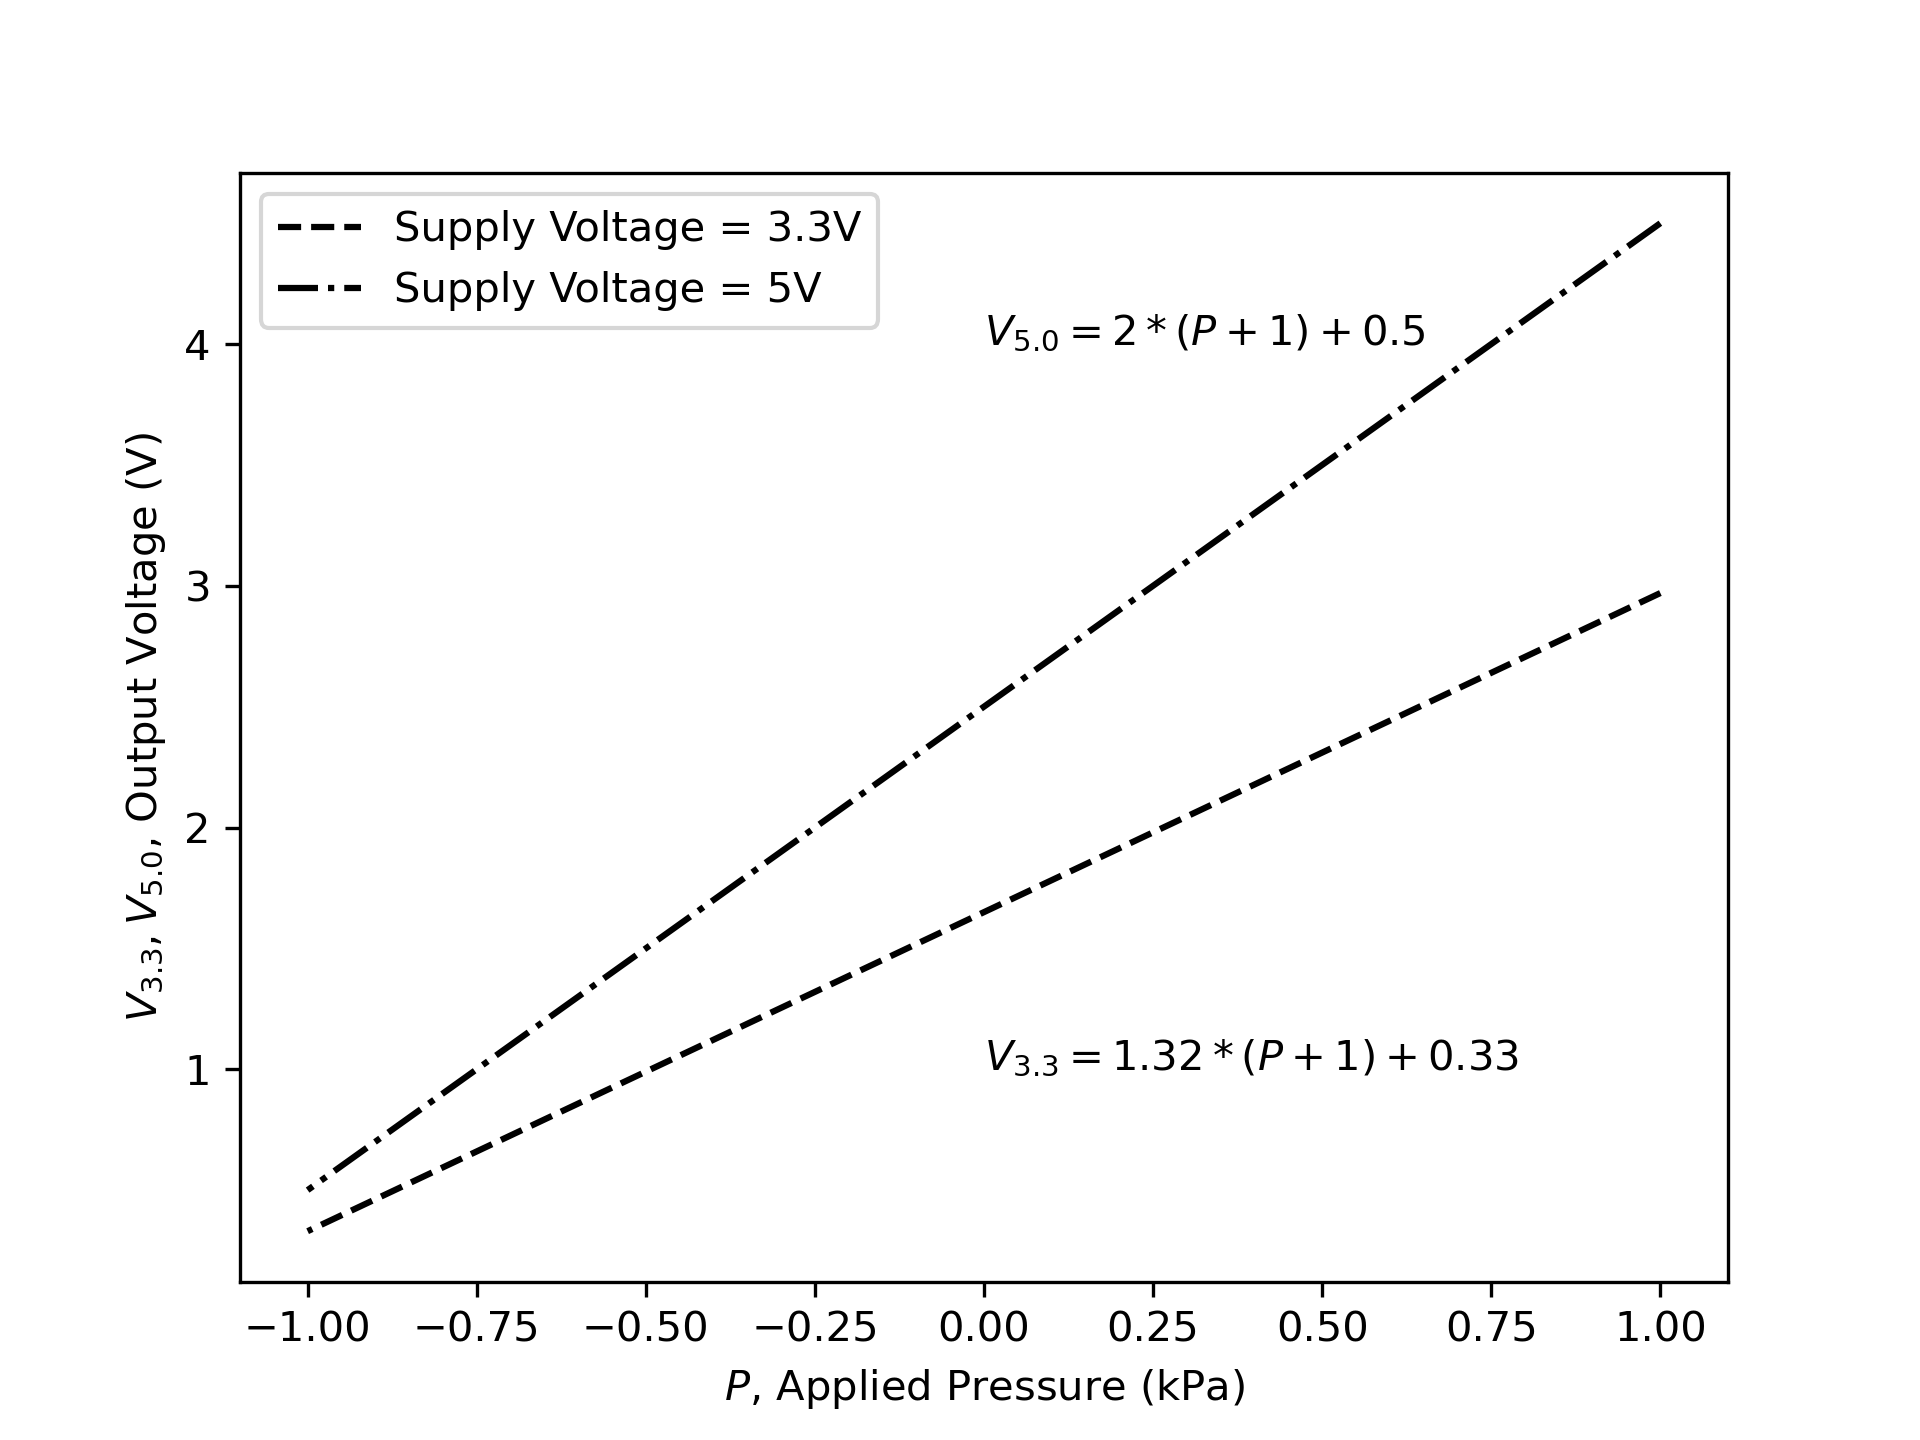
\includegraphics[width=0.8\linewidth]{matplotlib/q2VoltageOutputPlot.png}
    \caption{Voltage output of the sensor as a function of pressure over the range of the sensor if the supply voltage is 3.3 V and if it is 5V.}
    \label{fig:q2VoltageOutputPlot}
\end{figure}
The sensitivity of the sensor for each supply voltage is calculated by taking the derivative of the voltage output with respect to pressure. 
Since the equations for the voltage output are linear, the sensitivity is constant. 
\begin{empheq}[box=\fbox]{align*}
    \text{Sensitivity}_{3.3V} &= \frac{d}{dP} \left( 1.32*(P+1) + 0.33 \right) = 1.32 \text{ V/kPa} \\
    \text{Sensitivity}_{5V} &= \frac{d}{dP} \left( 2*(P+1) + 0.5 \right) = 2 \text{ V/kPa}
\end{empheq}

% plt.text(0, 1, '$V_{3.3} = 1.32*(P+1) + 0.33$')
% plt.text(0, 4, '$V_{5.0} = 2*(P+1) + 0.5$')

\section{}
The transfer function being used has an output range of 10\% to 90\% of the input range. That means the maximum output of the 
sensor is $0.9V_{\text{input}}$.

The voltage that the sensor outputs at $0.9$ kPa is not the maximum voltage. Determining that from the equations from Fig. \ref{fig:q2VoltageOutputPlot} gives:
\begin{align*}
    V_{3.3, \text{max}} &= 1.32(0.9+1) + 0.33 = \qty{2.838}{\volt} \\
    V_{5.0, \text{max}} &= 2(0.9+1) + 0.5 = \qty{4.3}{\volt} \\
\end{align*}
These values correspond to the maximum output of the sensor in practice. There is some wiggle room since the EDC can read up to 5V,
\begin{empheq}[box=\fbox]{align*}
    \text{Amplification}_{3.3\text{V}} &= \frac{V_{\text{EDC, max}} - V_{\text{EDC, min}}}{V_{3.3, \text{max}}} = \frac{5 - 0}{2.838} = 1.76 \\
    \text{Amplification}_{5.0\text{V}} &= \frac{V_{\text{EDC, max}} - V_{\text{EDC, min}}}{V_{5.0, \text{max}}} = \frac{5 - 0}{4.3} = 1.16
\end{empheq}
The resolution of the measurement systems are:
\begin{empheq}[box=\fbox]{align*}
    \text{Resolution}_{3.3\text{V}} &= \frac{V_{\text{EDC, max}} - V_{\text{EDC, min}}}{2^{n} G (\text{sensitivity}_{3.3V})} \\
    &= \frac{5 - 0}{2^{12} \times 1.76 \times 1.32} = \qty{5.2e-4}{\kilo\pascal} \\
    \text{Resolution}_{5.0\text{V}} &= \frac{V_{\text{EDC, max}} - V_{\text{EDC, min}}}{2^{12} G (\text{sensitivity}_{5V})} \\
    &= \frac{5 - 0}{2^{12} \times 1.16 \times 2} = \qty{5.2e-4}{\kilo\pascal}
\end{empheq}

\section{}
% 4) Read Page 3 and Page 13 of the data sheet. Determine the total bias 
% uncertainty in your system, in units of kPa, for each supply voltage (either 3.3 
% V or 5 V) using maximum amplification when the pressure transducer is 
% measuring 0.9 kPa when used in the temperature range of -20 to 85 oC. [3 
% marks] [Note: There is a bias uncertainty due to resolution of the A/D and a 
% bias uncertainty of the sensor].
At the operating temperature range of -20 to 85 $^\circ$C, the bias uncertainty of the sensor is $\pm 3.5\%$ FSS (Full Scale Span). Full scale,
as defined by the manufacturer, is the difference between the maximum and minimum output signals at the limits of pressure range.

The total bias uncertainty of the system is the RSS of the two independent uncertainties.

For the 3.3V supply voltage, the bias uncertainty of the sensor is:
\begin{align*}
    \text{Bias Uncertainty}_{3.3V} &= \% \text{err} \times \frac{\text{FSS}}{\text{sensitivity}} \\
    &= \pm 0.035 \times \frac{0.9\times3.3 - 0.1\times3.3}{1.32} = \qty{0.070}{\kilo\pascal}
\end{align*}
For the 5V supply voltage, the bias uncertainty of the sensor is:
\begin{align*}
    \text{Bias Uncertainty}_{5V} &= \% \text{err} \times \frac{\text{FSS}}{\text{sensitivity}} \\
    &= \pm 0.035 \times \frac{0.9\times5 - 0.1\times5}{2} = \qty{0.070}{\kilo\pascal}
\end{align*}

The bias uncertainty in kPa for 3.3V and 5V supply voltages are the exact same. In addition their resolutions are also the exact same. Calculating the
RSS for total uncertainty:
\begin{empheq}[box=\fbox]{align*}
    \delta P_{3.3\text{V}} = \delta P_{5.0\text{V}} &= \sqrt{\text{Quantization Uncertainty}^2 + \text{Bias Uncertainty}^2} \\
    &= \sqrt{(5.2 \times 10^{-4}/2)^2 + (7.0 \times 10^{-2})^2} = \qty{7.0E-2}{\kilo\pascal}
\end{empheq}
Observe that the bias uncertainty is much larger than the resolution of the system, and is the major contributor to the total uncertainty.
\section{}
% 5) State which supply voltage and amplification (if any) that should be used. [1 
% mark]. Is the cost and complexity of amplification worth the benefit of 
% increased resolution? [1 mark]. Why do you recommend the supply voltage 
% that you did? [1 mark] Is the uncertainty acceptable for this application? Why
% or why not? [1 marks]
The unamplified 5.0V system will be used.

The cost and complexity of amplification is not worth the small increased resolution. Additionally, the amplifier will introduce
additional error to the system.

The resolution of the unamplified 3.3V system ($5.2\times 10^{-4} \times 1.76 = \qty{9.2E-4}{\kilo\pascal}$) and the 5.0V system 
($5.2\times 10^{-4} \times 1.16 = \qty{6.0E-4}{\kilo\pascal}$), which are both reasonably close to the amplified system resolution of 
$\qty{5.2E-4}{\kilo\pascal}$. \textbf{Since an unamplified system is simpler, cheaper, and sufficiently resolving, the 5.0V system will be selected 
due to having a higher resolution than the 3.3V system.}

The uncertainty for this system is $\delta P_{5.0\text{V}} = \qty{7.0E-2}{\kilo\pascal}$, which is an order of magnitude smaller than the 
highest pressure measured. This should be sufficient for the application of the sensor.

\section{}
% 6) Rapid pressure fluctuations can occur in the engine intake, which may disrupt 
% your measurements. Recommend a method so that these fluctuations do not 
% disrupt your measurement. [1 mark]
% Note: 3 Marks will be given based on the clarity of the presentation of your calculations 
% and discussion
Since the design is concerned with sustained (lower frequency) pressures, a low-pass filter can be used to filter out the higher frequency
signals. 

Transform the signal into the frequency domain using FFT, then employ a low-pass filter as the transfer function. Then 
inverse transform the signal back into the time domain to obtain the filtered signal!

